\chapter{Analysis and methodology}
\label{ana-meth}

\section{Time series forecasting - general model structure}
A model for time series forecasting must be structured in the following way.
As input, it must take a sequence of vectors, with each vector representing a single point in time, and each element of the vector representing an element of the multivariate time series.
For example, a multivariate time series of load and temperature would be represented by a sequence of vectors, each with two elements.
As output, the system must similarly produce a sequence of multivariate vectors.
In the case that the model is forecasting only a single time series, the output vectors will have only a single element each.
This structure is presented in Figure \ref{fig:forecast-model}.
Of course, it may be the case that a time series forecasting model is comprised of several models cascaded together.
Perhaps the sequence of input vectors are concatenated by one model, then passed to the actual forecasting model which produces a single output vector, then the output vector is split by a third model before being produced at the output.

\begin{figure}
	\centering
	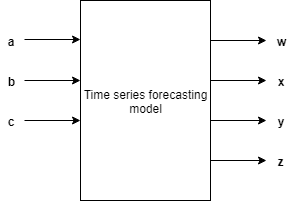
\includegraphics[width=0.35\linewidth]{images/forecast-model}
	\caption{A time series forecasting model takes a sequence of vectors, $\va, \vb, \vc$, as input and produces a sequence of vectors, $\vw, \vx, \vy, \vz$, as output. Note the number of input and output vectors is able to vary.}
	\label{fig:forecast-model}
\end{figure}

This structure - with sequences of input and output vectors - is identical to that used for neural machine translation (NMT), where a source sentence/phrase is translated from one language, say English, to another language such as Dutch \citep{Cho2014}.
In NMT, a word is represented by a vector, and a sentence is represented by a sequence of vectors.

\par
This section will investigate the performance of several of the best performing NMT architectures when applied to time series forecasting.
\hl{I'm still deciding whether I want to put the evaluation before I discuss in detail how the architectures work.
	Benefit of putting evaluation first is that it prevents the reader from being daunted by too much detail upfront.
	Might seem a little backwards though.}

\section{Investigated models and methods}
The following models will be discussed and their results in time series forecasting compared.
\begin{itemize}
	\item ARIMA
	\item Sequence to sequence (S2S) recurrent neural network (RNN) \citep{Cho2014a} using long short term memory (LSTM) \citep{hochreiter1997long} cells
	\item Transformer \citep{Vaswani2017}
	\item Universal Transformer \cite{Dehghani2018}
	\item Clio - a modified transformer with the ability to automatically select similar profile data
\end{itemize}

Additionally, a similar profile selection method was developed to provide the models with relevant input data.
These models and methods are described in the following sections.

\section{ARIMA}
blah

\section{Recurrent neural network}
Introduce RNN, then within this same section expand it to include sequence to sequence architecture, and then again expand it to include attention mechanisms.

\section{Transformer}
\hl{My preliminary investigations show that the transformer architecture is the best, or at least equal best but likely with less expensive training. This is consistent with \protect\cite{Song2017} and \protect\cite{Vaswani2017}}\\
\par
The transformer is a neural network architecture that is currently the state of the art in NMT \citep{Vaswani2017}.
This architecture will be discussed in detail. 

\subsection{Overview}
overview of the transformer architecture.
\begin{itemize}
	\item encoder and decoder
	\item input embedding
	\item positional encoding
	\item multi-head attention
	\item residual connections
	\item feed forward
	\item layer normalization
	\item 
\end{itemize}

\subsection{Input embedding}
convolutional embedding as per \citep{Song2017} (a paper using the transformer architecture to perform classification based on time series).

\subsection{Positional encoding}
Every input vector, $\vb_i$, has a vector added to it, $\vp_i$, depending on its position, $i$, in the input.
$\vp_i$ is trainable - it is drawn from $\vtheta$.

\subsection{multi-head attention}
I need to research this further before writing about it.

\subsection{residual connections}

\subsection{Feedforward}

\subsection{Normalization}

\subsection{etc.}

\subsection{Training}
Discuss how the decoder is used in training and inference modes.
Causality, iterative inference.

\section{Universal Transformer}
blah

\section{Clio}
blah

\section{Similar profile selection}
Load profiles are influenced by exogenous data such as weather, day of the week, and holiday type \cite{Weron2006}.
A simple and intuitive method of load forecasting is to find periods in the past with similar exogenous data to the period being forecast and then use the load profiles from these past periods to form a forecast \cite{Senjyu1998}.
However, these similar period methods can be insufficient to capture complex patterns, especially over holiday periods which occur only once per year \cite{Chen2010}.

%Holiday type indicates which holiday the load profile occurs on - Easter or Christmas for example.
%These different holidays are assigned different integer identifiers (with normal days assigned identifier 0) to form a time series.

The forecasting system was provided with historical load and weather profiles from periods that had similar exogenous data to the period of the load profile being forecast.
Similar periods were identified by first finding candidate similar periods an integer multiple of 1 year $\pm$30 days away from the period being forecast.
These candidates were then filtered down to periods with exactly matching hour and minute.

Then the weighted Euclidean distance between the period being forecast and each candidate similar period was calculated using the following features: 
maximum future temperature, 
minimum future temperature,
maximum past load,
current holiday type, 
current day of the week,
current day of the month, and
current month of the year.
The holiday type indicates the current holiday --- Easter or Christmas for example --- and is encoded as a time series of integers with a different integer for each holiday.
When the holiday type always occurs on the same date each year then the month of the year and day of the month were used, whereas when the holiday type always occurs on the same day of the week each year then the day of the week was used.
The candidate similar periods with the lowest Euclidean distance were selected as the final set of similar periods.

When training and testing the model the similar periods were selected from both the past and the future, as the train and test datasets were only five years each.
It was assumed that, for testing, there were no changes in the patterns underlying the load profile over the duration of the testing set.

\section{Evaluation tasks}
The following time series forecasting tasks will be used to evaluate the models
\begin{itemize}
	\item forecasting a pure sine wave given its past values
	\item forecasting a sine wave with normally distributed noise given its past values
	\item forecasting a signal comprised of several sine waves with normally distributed noise given past values
	\item forecasting the Bruny Island load data - no priority given to special days.
\end{itemize}

\section{Evaluation Results}
\hl{At this stage, only performance on the actual load forecasting task has been evaluated} \\
with the following notation: \\
$L$ number of hidden layers \\
$h_d$ dimension of the state vector \\
$A$ number of attention units \\
$h_a$ dimension of attention state vector


\begin{table}[htbp]
	\centering
	\begin{tabular}{lcl}
		\hline
		\textbf{Architecture} & \textbf{Loss} & \\
		\hline
		Transformer with 256 hidden units, 4 heads, 4 layers   &  -5.85  &  \\
		S2S GRU with  $L = 2, h_d = 5, A=2, h_a=5$ &  -5.72  &  \\
		S2S GRU with  $L = 2, h_d = 5, A=2, h_a=0$  &  -5.75  &  \\
		S2S GRU with  $L = 2, h_d = 5, A=0, h_a=0$  &  -5.65  &  \\
		S2S LSTM with  $L = 2, h_d = 5, A=0, h_a=0$  &  -5.66  &  \\
		\hline
	\end{tabular}
	\caption{Comparison of architectures evaluated so far.}
	\label{tab:architecture_comparison}
\end{table}

Preliminary forecasting results are displayed in section \ref{bruny-results}.
It must be noted that not all architectures have been tuned as well as they could.



	